\documentclass[10pt, landscape]{article}
\usepackage[scaled=0.92]{helvet}
\usepackage{calc}
\usepackage{multicol}
\usepackage{ifthen}
\usepackage[a4paper,margin=5mm,landscape]{geometry}
\usepackage{amsmath,amsthm,amsfonts,amssymb}
\usepackage{color,graphicx,overpic}
\usepackage{hyperref}
\usepackage{newtxtext} 
\usepackage{enumitem}
\usepackage{amssymb}
\usepackage[table]{xcolor}
\usepackage{vwcol}
\usepackage{tikz}
\usetikzlibrary{arrows.meta}
\usetikzlibrary{calc}
\usepackage{mathtools}
\usepackage{nicematrix}
\usepackage[T1]{fontenc} %%% <--- NOTE THIS
% for relations
\usepackage{cancel}
\usepackage{ mathrsfs }
\usepackage{listings}
\usepackage{background}
\setlist{nosep}

\backgroundsetup{
scale=1,
color=black,
opacity=0.4,
angle=0,
contents={%
  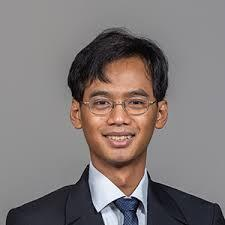
\includegraphics[width=\paperwidth,height=\paperheight]{prof.jpg}
  }%
}

\pdfinfo{
  /Title (CS2030S.pdf)
  /Creator (TeX)
  /Producer (pdfTeX 1.40.0)
  /Author (Seamus)
  /Subject (Example)
  /Keywords (pdflatex, latex,pdftex,tex)}

\lstset{language=Java,keywordstyle={\bfseries \color{black}}}

% Turn off header and footer
\pagestyle{empty}

\newenvironment{tightcenter}{%
  \setlength\topsep{0pt}
  \setlength\parskip{0pt}
  \begin{center}
}{%
  \end{center}
}

% redefine section commands to use less space
\makeatletter
\renewcommand{\section}{\@startsection{section}{1}{0mm}%
                                {-1ex plus -.5ex minus -.2ex}%
                                {0.5ex plus .2ex}%x
                                {\normalfont\large\bfseries}}
\renewcommand{\section}{\@startsection{section}{2}{0mm}%
                                {-1explus -.5ex minus -.2ex}%
                                {0.5ex plus .2ex}%
                                {\normalfont\normalsize\bfseries}}
\renewcommand{\subsection}{\@startsection{subsection}{3}{0mm}%
                                {-1ex plus -.5ex minus -.2ex}%
                                {1ex plus .2ex}%
                                {\normalfont\small\bfseries}}%
\renewcommand{\familydefault}{\sfdefault}
\renewcommand\rmdefault{\sfdefault}
% makes nested numbering (e.g. 1.1.1, 1.1.2, etc)
\renewcommand{\labelenumii}{\theenumii}
\renewcommand{\theenumii}{\theenumi.\arabic{enumii}.}
\renewcommand\labelitemii{•}
%  for logical not operator
\renewcommand{\lnot}{\mathord{\sim}}
\renewcommand{\bf}[1]{\textbf{#1}}
\newcommand{\abs}[1]{\vert #1 \vert}
\newcommand{\Mod}[1]{\ \mathrm{mod}\ #1}

\makeatother
\definecolor{myblue}{cmyk}{1,.72,0,.38}
\everymath\expandafter{\the\everymath \color{myblue}}
% Define BibTeX command
\def\BibTeX{{\rm B\kern-.05em{\sc i\kern-.025em b}\kern-.08em
    T\kern-.1667em\lower.7ex\hbox{E}\kern-.125emX}}
\let\iff\leftrightarrow
\let\Iff\Leftrightarrow
\let\then\rightarrow
\let\Then\Rightarrow

% Don't print section numbers
\setcounter{secnumdepth}{0}

\setlength{\parindent}{0pt}
\setlength{\parskip}{0pt plus 0.5ex}
%% this changes all items (enumerate and itemize)
\setlength{\leftmargini}{0.5cm}
\setlength{\leftmarginii}{0.5cm}
\setlist[itemize,1]{leftmargin=2mm,labelindent=1mm,labelsep=1mm}
\setlist[itemize,2]{leftmargin=4mm,labelindent=1mm,labelsep=1mm}

%My Environments
\newtheorem{example}[section]{Example}
% -----------------------------------------------------------------------

\begin{document}
\raggedright
\footnotesize
\begin{multicols*}{4}


% multicol parameters
% These lengths are set only within the two main columns
\setlength{\columnseprule}{0.25pt}
\setlength{\premulticols}{1pt}
\setlength{\postmulticols}{1pt}
\setlength{\multicolsep}{1pt}
\setlength{\columnsep}{2pt}

\begin{center}
    \fbox{%
        \parbox{0.8\linewidth}{\centering \textcolor{black}{
            {\Large\textbf{CS2030S}}
            \\ \normalsize{AY24/25 Sem 1}}
            \\ {\footnotesize \textcolor{myblue}{by ngmh}} 
        }%
    }
\end{center}

\section{Programming Languages}
\begin{itemize}
\item Dynamic v/s Static Typing: Dynamic languages have variables that can hold values of multiple different unrelated types. Static languages have variable types that must be declared and cannot be changed \\
\item Strong v/s Weak Typing: Stronger languages have greater rules in their type system to ensure type safety
\end{itemize}

\section{Tombstone Diagram}
\begin{center}
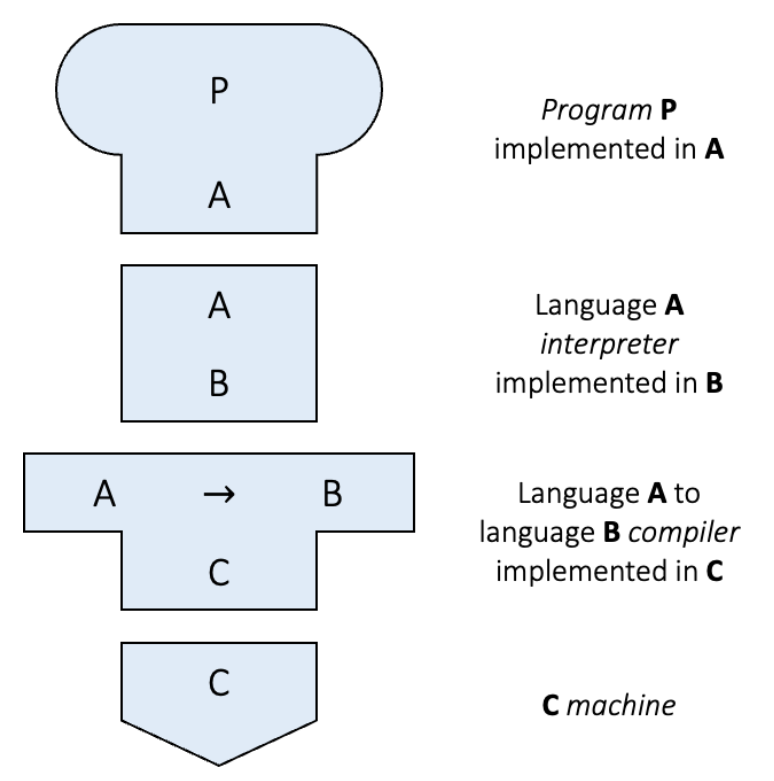
\includegraphics[width=0.5\linewidth]{tombstone.png}
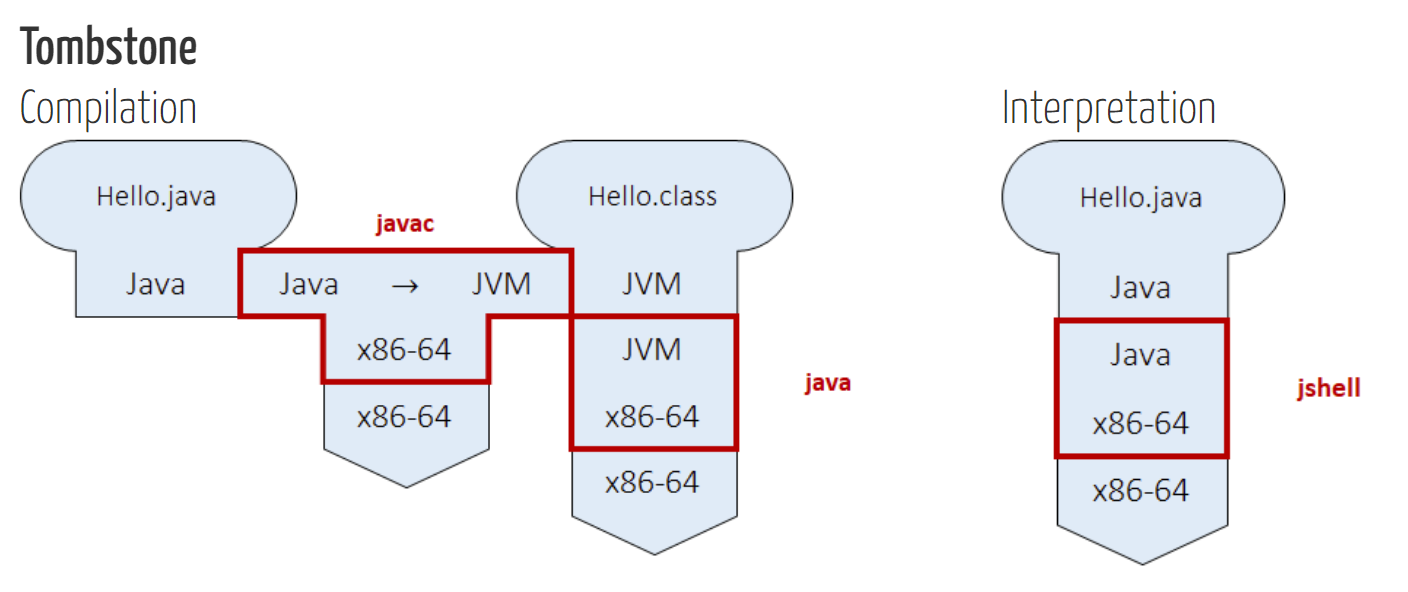
\includegraphics[width=\linewidth]{java.png}
\end{center}

\section{Java Subtyping and Types}
\begin{itemize}
\item T is a subtype of S (T <: S) if code written for S can be safely used for T \\
\item T has a narrower scope, while S has a wider scope \\
    \begin{itemize}
        \item T can be put into S (widening) \\
        \item S can be explicitly typecast into T (narrowing) \\
    \end{itemize}
\item{Primitive Types}
\begin{itemize}
    \item byte <: short <: int <: long <: float <: double \\
    \item char <: int
\end{itemize}
\item{Reference Types}
\begin{itemize}
    \item Anything that is not a Primitive Type such as classes
    \item Stores only a reference to the value, like a pointer
    \item Two reference variables can share the same value; $==$ compares references not actual values
    \item Default null value, which could cause errors
\end{itemize}
\end{itemize}

\section{Class Fields and Methods}
\begin{itemize}
    \item Use the \verb|static| keyword to specify
    \item Access using \verb|Class.field| or \verb|Class.method()|
    \item \verb|this| keyword will NOT work in Class Methods.
\end{itemize}

\section{Pillars of OOP}
\begin{itemize}
    \item Encapsulation: Bundle of variables (fields) and functions (methods), by making a \verb|class|, that can be represented in a class diagram
    \item Abstraction: Writing reusable code by grouping sets of instructions
    \item (Not a Pillar) Composition: Creating wrapper class around an object with additional fields, models a \textbf{Has-A} relationship
    \item Inheritance: Preserve methods and fields of the original object, models a \textbf{Is-A} relationship
    \item Polymorphism: Allowing one variable to take on different run-time types, or different methods to be called
\end{itemize}

\section{OOP Style}
\begin{itemize}
    \item Information Hiding:
    \begin{itemize}
        \item Mark fields as \verb|private| where possible. Objects of same class can still access them.
        \item Avoid having a \textbf{getter} or \textbf{setter} when possible
    \end{itemize}
    \item Tell Don't Ask: Client should tell the class what to do, rather than gathering information to manually calculate
\end{itemize}

\section{Stack and Heap}
\begin{itemize}
    \item Stack:
        \begin{itemize}
            \item Where all variables are allocated and stored
            \item Contains \textbf{Call Frames}, which are created and destroyed when methods are called
        \end{itemize}
    \item Heap:
        \begin{itemize}
            \item Where objects are allocated and stored
            \item \lstinline{new} is used: Object created on heap
            \item Objects are stored as Class Name, Instance Fields and Values, and Captured Variables
        \end{itemize}
    \item Example Diagram when \verb|distanceTo()| is called
    \begin{lstlisting}
    Point p1 = new Point(0, 0);
    Point p2 = new Point(1, 1);
    p1.distanceTo(p2);
    \end{lstlisting}
    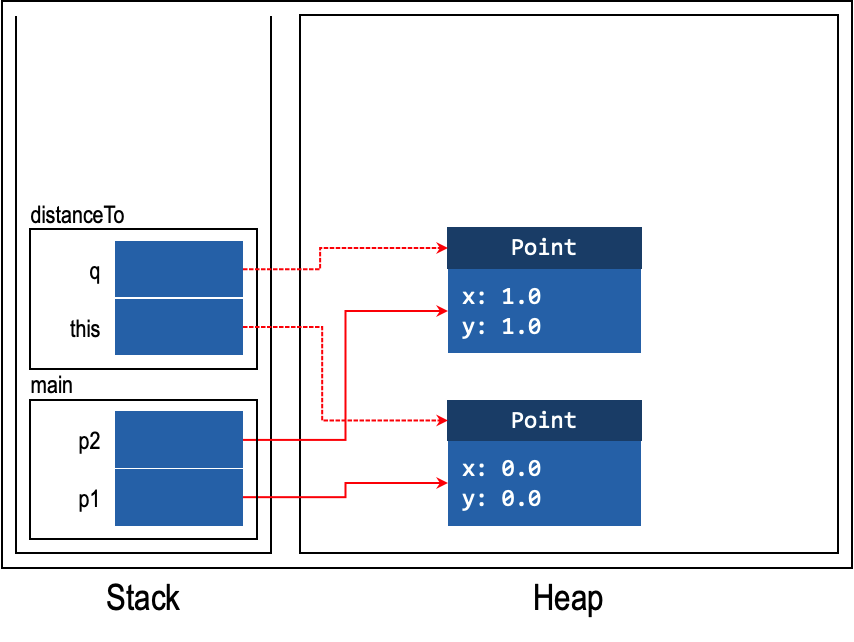
\includegraphics[width=\linewidth]{006b.png}
\end{itemize}

\section{Inheritance}
\begin{itemize}
    \item Use the \verb|extends| keyword
    \item Parent Constructor: \verb|super()|, \textbf{ONLY FIRST LINE}
    \item Overriding
    \begin{itemize}
        \item Use the \lstinline{@Override} annotation
        \item Match \textbf{Method Descriptor} (Name of method, Type of Parameters, Return Type), can't throw new exceptions
    \end{itemize}
    \item Overloading
    \begin{itemize}
        \item Method with same name but different \textbf{Method Signature} (Name of method, Type of Parameters)
    \end{itemize}
    \item Liskov Substitution Principle
    \begin{itemize}
        \item Any property of objects of type T should be true for any object of type S where S <: T
        \item Don't break expectations of the parent class
    \end{itemize}
\end{itemize}

\section{Dynamic Binding}
\begin{itemize}
    \item Compile Time Type v/s Run Time Type
    \begin{itemize}
        \item \verb|Circle c = new ColouredCircle()|
        \item CTT(c) = Circle, RTT(c) = ColouredCircle
    \end{itemize}
    \item Example: \verb|obj.foo(arg)|
    \item Compile Time
    \begin{itemize}
        \item Check CTT(obj) and CTT(arg)
        \item Find all accessible methods named \verb|foo|, including those in supertypes of CTT(obj)
        \item Find most specific method (narrowest) that fits with CTT(arg)
        \item Record the method descriptor
    \end{itemize}
    \item Run Time
    \begin{itemize}
        \item Retrieve method descriptor
        \item Determine RTT(obj), recursing upwards to find first method fitting descriptor
    \end{itemize}
    \item Does not apply to Class methods
\end{itemize}

\section{Abstract Classes}
\begin{itemize}
    \item A general class, that should \textbf{NEVER} be instantiated
    \item Use the \verb|abstract| keyword
    \item Abstract arrays can still be defined
    \item Abstract methods do not have any body
    \item A class with abstract methods must be made abstract
\end{itemize}

\section{Interface}
\begin{itemize}
    \item Models requirements of classes
    \item Use the \verb|implements| keyword for inheritance, methods are public abstract by default
    \item A class can implement multiple interfaces
    \item Solves Diamond Problem:
    \begin{itemize}
        \item If inheritance from multiple classes were allowed, there could be conflicting method declarations
        \item Can satisfy both at once with pure interfaces
    \end {itemize}
    \item Casting to interfaces is allowed, since class could satisfy without explicitly implementing
    \item Impure interface: Has method body with \verb|default| keyword
\end{itemize}

\section{Wrapper Classes}
\begin{itemize}
    \item Encapsulate primitive types
    \item Auto-boxing: Automatically put primitive types into wrapper class (line 1); Auto-unboxing: Automatically put value of wrapper class into primitive variable (line 2)
    \begin{lstlisting}
    Integer i = 4;
    int j = i;
    Double d = 2;
    \end{lstlisting}
    \item However, 2 step boxing is not allowed, (line 3: 2 is not automatically casted to a double before auto-boxing)
    \item Wrapper classes \textbf{DO NOT} share the same subtyping relationship as primitives
    \item Using wrapper classes come at a performance cost, as objects have to be stored on the heap
    \item Wrapper classes are immutable, changing value involves auto-boxing and auto-unboxing to make a new object
\end{itemize}

\section{Type Checking}
\begin{itemize}
    \item \verb|a = (C) b|
    \item Compile Time
    \begin{itemize}
        \item Find CTT(b), then check if it is possible for RTT(b) <: C, if not Compile Error
        \item Possibility:
        \begin{itemize}
            \item CTT(b) <: C: This widening cast is allowed
            \item C <: CTT(b): This narrowing cast requires runtime checks for RTT(b)
            \item C is an interface: There could be a subclass of B implementing C, so a runtime check is needed
        \end{itemize}
        \item Impossibility:
        \begin{itemize}
            \item B and C are unrelated
            \item C is an interface and B is final
        \end{itemize}
        \item Find CTT(a), then check if C <: CTT(a), if not Compile Error
        \item Add run-time check for RTT(b) <: C
    \end{itemize}
    \item Run Time
    \begin{itemize}
        \item Find RTT(b), then check if RTT(b) <: C
    \end{itemize}
\end{itemize}

\section{Variance}
\begin{itemize}
    \item Java Arrays are Covariant: S <: T implies S[] <: T[]
    \item Contravariant: S <: T implies (T) <: (S)
    \item Invariant: None of the above, not comparable
\end{itemize}

\section{Exceptions}
\begin{itemize}
    \item Use \verb|try catch finally| keywords
    \item \verb|throw| immediately suspends execution of the \verb|try| block
    \item \verb|catch| can catch all exceptions which are subtypes
    \item \verb|finally| \textbf{ALWAYS RUNS}, unless computer explodes
    \item Exceptions can be thrown upwards using \verb|throws|
    \item Unchecked Exceptions: Caused by programming errors, not explicitly caught or thrown, subclasses of RTE
    \item Checked Exceptions: Beyond programmer's control, must be actively anticipated and handled if not program will not compile
\end{itemize}

\section{Generics}
\begin{itemize}
    \item Generic Types can take in Type Parameters
    \item Can be bounded by classes and interfaces using \verb|extends|
    \item Do not use 2 parameters of the same name together
    \item Note that generics are \textbf{invariant}
    \item Example Usage
\end{itemize}
\begin{lstlisting}
    class Pair<S, T>{} // Definition
    <T> boolean contains(T[] array, T obj){}
    A.<String>contains(strArr, str) // Usage
\end{lstlisting}

\section{Type Erasure}
\begin{itemize}
    \item Java thing for backwards compatibility
    \item Generic types are replaced by their upper bound, e.g. Comparable (default Object)
    \item When a Generic is instantiated and used, a typecast is added to the code
\end{itemize}
\begin{lstlisting}
    Int i = new Pair<Str,Int>("a", 4).sec();
    Int i = (Int) new Pair("a", 4).sec();
\end{lstlisting}

\section{Generic Array Problems}
\begin{itemize}
    \item Due to type erasure, we cannot tell if putting Generics into an array will cause errors
    \item See code below:
\end{itemize}
\begin{lstlisting}
    Pr<Str, Int>[] pArr = new Pr<Str, Int>[2];
    Object[] oArr = pArr;
    oArr[0] = new Pr<Dbl, Bool>(3.14, true);
\end{lstlisting}
\begin{itemize}
    \item becomes
\end{itemize}
\begin{lstlisting}
    Pr pArr = new Pr[2];
    Object[] oArr = pArr;
    oArr[0] = new Pr(3.14, true);
\end{lstlisting}
\begin{itemize}
    \item and this looks okay to us now
    \item But if we do \verb|Str str = pArr[0].first()|, we get a \lstinline{ClassCastException}
    \item Arrays are reifiable, with full type information available at run-time, unlike generics, so Java does not allow this
    \item Array declaration is ok, but instantiation with \verb|new| is not
\end{itemize}

\section{Generic Type Rules}
\begin{itemize}
    \item Generic method signature includes type parameters, with them being equal up to renaming
    \item Type checking uses type argument for class-level type parameters where possible
    \item Method descriptor stored during dynamic binding at CTT is type erased
\end{itemize}

\section{Generic Arrays and Warnings}
\begin{itemize}
    \item Since we cannot instantiate generic arrays, we typecast it instead, since arrays are covariant
\end{itemize}
\begin{lstlisting}
    T[] tmp = (T[]) new Object[sz];
    this.arr = tmp;
\end{lstlisting}
\begin{itemize}
    \item Generates warning, can view with \verb|-Xlint:unchecked|
    \item Compiler cannot guarantee absence of RTE, due to possible modification
    \item Can suppress with \verb|@SuppressWarning("unchecked")|, but need to justify it
    \item Another warning is for raw types, where compiler cannot guarantee type safety due to usage of raw types
\end{itemize}

\section{Wildcards}
\begin{itemize}
    \item Solves problem with generics being invariant
    \item Upper-Bounded: Covariant; S <: T implies <? extends S> <: <? extends T>, <S> <: <? extends S>
    \item Lower-Bounded: Contravariant; S <: T implies <? super T> <: <? super S>, <S> <: <? super S>
    \item PECS: Produce Extends, Consumer Super
    \begin{itemize}
        \item Think from perspective of the wildcard
        \item In copyFrom, the wildcard is producing a value
        \item In copyTo, the wildcard is consuming a value
    \end{itemize}
    \item Unbounded Wildcards: "Supertype" of all wildcards
    \begin{itemize}
        \item Use to replace raw types, does not produce any warnings as no (nonexistent) type information is lost
    \end{itemize}
\end{itemize}

\section{Type Inference}
\begin{itemize}
    \item Can use an empty diamond operator on RHS to instantiate generic types; useful if generic type is really long
    \item 3 Step Method:
    \begin{itemize}
        \item Argument Typing: Type of parameters passed in
        \item Target Typing: Type of variable where return is stored
        \item Type Parameter: Self explanatory
    \end{itemize}
    \item Only consider types explicitly involved then choose the most specific type
    \item Example
\end{itemize}
\begin{lstlisting}
    <T extends Circle> T f(Seq<? super T> s)
    GetAreable c = f(new Seq<Circle>());
\end{lstlisting}
\begin{itemize}
    \item Type Inference
    \begin{itemize}
        \item Argument Typing: Circle super T, T <: Circle
        \item Target Typing: GetAreable c = T, T <: GetAreable
        \item Type Parameter: T extends Circle, T <: Circle
    \end{itemize}
    \item Resolved as T <: Circle, so T is Circle
\end{itemize}

\section{Factory Methods}
\begin{itemize}
    \item Create classes through factory rather than constructor
    \item Static method, hides constructor information
    \item Useful when consumer does not know exactly what subtype should be created, acts as auxiliary
    \item Capture generic types to correctly parameterise
\end{itemize}

\section{Immutability}
\begin{itemize}
    \item Use the \verb|final| keyword to prevent inheritance of classes, or modification of methods, or re-assignment of fields.
    \item Ensure types of fields are immutable.
    \item Ensure arrays are copied before assignment.
    \item Ensure there no mutators, return new instance instead.
    \item \textbf{@SafeVarargs}: Allow different kinds of parameters in constructor such as multiple numbers of number array.
\end{itemize}

\section{Nested Classes}
\begin{itemize}
    \item Capture super class if not static
    \item Example: B and C are nested, but C and y are static
\end{itemize}
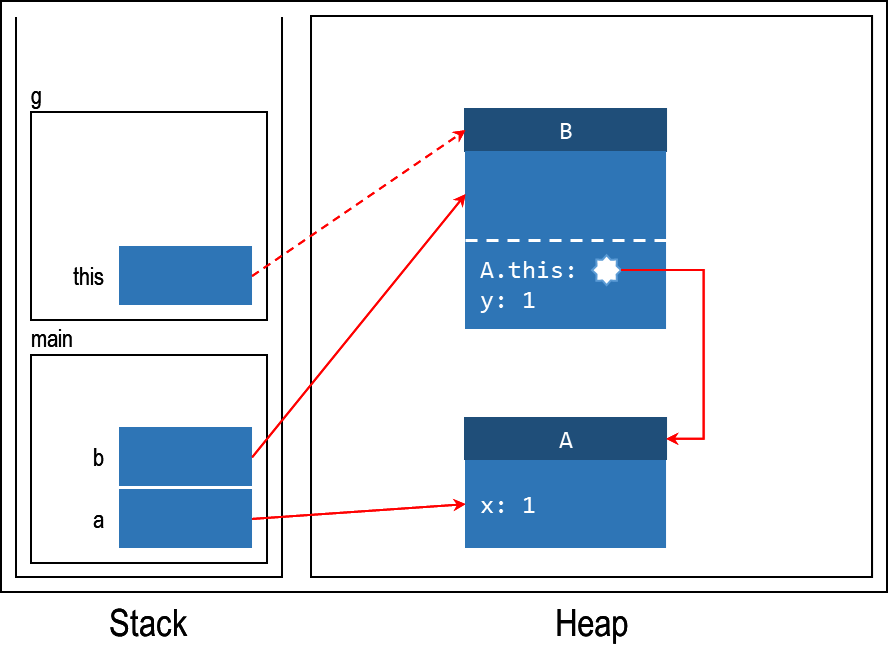
\includegraphics[width=\linewidth]{010f.png}
\begin{itemize}
    \item Local Class: Class within a function, access enclosing class fields with this
    \item Effectively final for primitive types (cannot be reassigned), makes copies of local variables when capturing
    \item Anonymous Class: Declare and instantiate local class in the same statement
\end{itemize}

\section{Side Effect-Free Programming and Lambdas}
\begin{itemize}
    \item Side Effect: Printing, Modifying value of field, Mutating arguments, throwing exceptions, etc.
    \item Referential Transparency: Can replace every $f(x)$ with $y$ in code. Function must be deterministic.
    \item Pure Function: Side-effect free, Referentially Transparent.
    \item Inline Functions in Java are implemented as methods in anonymous classes that implements an interface, and will show in the Stack and Heap.
    \item \textbf{@FunctionalInterface} has exactly one abstract method.
    \item Lambdas using Method References for Static Method, Instance method, and Constructor:
\end{itemize}
\begin{lstlisting}
Maybe::of // x -> Maybe.of(x)   
x::compareTo // y -> x.compareTo(y)
Some::new // x -> new Some(x)
\end{lstlisting}
\begin{itemize}
    \item This can be confusing when there are multiple parameters for a \verb|A::h|, as it could be either class or instance method:
\end{itemize}
\begin{lstlisting}
// 2: (x, y) -> x.h(y) or A.h(x, y)
// 3: (x, y, z) -> x.h(y, z) or A.h(x, y, z)
\end{lstlisting}
\begin{itemize}
    \item When using lambdas, captured variables are effectively final, unlike when using method references.
    \item Currying: Returning a lambda from a function. Instance methods can be seen as partially applied curried functions.
\end{itemize}

\section{Maybe and Lazy}
\begin{itemize}
    \item Internalise null checks to prevent bugs.
    \item Mutate content using transformers, not instance methods.
    \item Using lambdas, we can define functions for later execution.
    \item Memoization: Cache the result after evaluation.
\end{itemize}

\section{Monads and Functors}
\begin{itemize}
    \item Monad: Class with a value and additional side information. Has the \verb|of|, \verb|map| and \verb|flatMap| methods.
    \item Monadic Laws
    \begin{itemize}
        \item Left Identity Law: \verb|Monad.of(x).flatMap(x -> f(x)| is the same as \verb|f(x)|.
        \item Right Identity Law: \verb|x.flatMap(y -> Monad.of(y))| is the same as \verb|x|.
        \item Associative Law: \verb|x.flatMap(y -> f(y)).flatMap(y -> g(y))| is the same as \verb|x.flatMap(y -> f(y).flatMap(z -> g(z)))|.
    \end{itemize}
    \item Functor: Ensures lambdas can be applied sequentially without worrying about side information.
    \begin{itemize}
        \item Identity Law: \verb|x.map(y -> y)| is the same as \verb|x|.
        \item Composition Law: \verb|x.map(y -> f(y)).map(y -> g(y))| is the same as \verb|x.map(y -> g(f(y))|.
    \end{itemize}
\end{itemize}

\section{InfiniteList and Streams}
\begin{itemize}
    \item Simple linked list: Store content as head, next node as tail.
    \item For infinite length, need to evaluate lazily.
    \item Java Streams are infinite lists with more functionalities.
    \item Terminal Operation: Triggers evaluation of stream.
    \item Intermediate Operation: Returns another Stream.
    \item Bounded Operations: Operations that should only be called on finite streams. They can be stateful, requiring some form of keeping track of states to operate.
    \item Truncation: Use functions like \verb|limit| or \verb|takeWhile|.
    \item A Stream can only be operated on once.
\end{itemize}

\section{Parallelism and Concurrency}
\begin{itemize}
    \item Concurrency: Switching rapidly between multiple tasks to making it seem like they are running at the same time.
    \item Parallelism: Running subtasks on multiple cores so that they are actually executed at the same time.
    \item Stream: Use \verb|.parallel()|. Order is not preserved.
    \item Embarrassingly Parallel: Only involve one element at once.
    \item Stateful operations or those with side effects might produce the wrong result when parallelised.
    \item Parallelising \verb|reduce(id, acc, comb)|:
    \begin{itemize}
        \item \verb|comb.apply(id, i)| must equal \verb|i|.
        \item Combiner must be associative. Some non-associative accumulators also work, depending on usage.
        \item Accumulator and Combiner must be compatible: \verb|comb.apply(u, acc.apply(id, t))| must equal \verb|acc.apply(u, t)|.
    \end{itemize}
\end{itemize}

\section{Threads and Asynchronous Programming}
\begin{itemize}
    \item Normally, operations are blocking; code execution only resumes once the operation is finished.
    \item Threads are a simple flow of execution in a program. We can create them programmatically to run two things at the same time. The \verb|.start()| method returns instantly.
    \item Using and managing Threads is complicated.
    \item \verb|CompletableFuture<>| is a monad that allows us to perform tasks concurrently. It has methods like \verb|allOf| or \verb|thenApply| to make composition and mapping easy.
    \item Multiple \verb|thenApply|s, are evaluated as a stack (LIFO).
    \item To get the result, we have to use \verb|.get()|, or \verb|.join()| (doesn't throw checked exceptions).
    \item Java uses thread pools to manage threads through \verb|ForkJoinPool|.
    \begin{itemize}
        \item Each thread has a deque of tasks.
        \item When a thread is idle, it checks its deque of tasks. If not empty, it takes the head task to execute using \verb|.compute()|. Otherwise, it takes the tail task of another deque to run (work stealing).
        \item When \verb|.fork()| is called, the caller adds itself to the head of the deque of the executing thread. Subsequent forks also add to the head of the deque, like recursion.
        \item When \verb|.join()| is called, if the subtask to be joined hasn't been executed, \verb|.compute()| is called and it is executed. If it has been completed, the result is read and \verb|.join()| returns. If the subtask has been stolen, the current thread finds other tasks to work on.
        \item Forks and joins should be called in a palindromic manner. The most recently forked task should be the first to be joined. There should also be at most one compute in the middle. This is because if a task is joined when it is not at the head, we have to search through the deque to find and execute it.
    \end{itemize}
\end{itemize}

\begin{center}
    \begin{tabular}{lll}
    \raisebox{-.5\height}{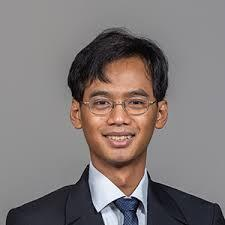
\includegraphics[scale=0.25]{prof.jpg}} & pls give me A+ prof thanks \\
    \end{tabular}
\end{center}

\end{multicols*}

\end{document}